\documentclass[a4paper]{article}

\usepackage[english]{babel}
\usepackage[utf8]{inputenc}
\usepackage[final]{graphicx}
\usepackage{subcaption}
\usepackage{amsmath}
\usepackage{graphicx}
\usepackage[colorinlistoftodos]{todonotes}
\usepackage{listings}

\title{Applikationsutveckling med Ionic \\ Stockholm B\&B }

\author{Alice Darner}

\date{\today}

\begin{document}
\maketitle

\begin{abstract}
En en enkel hotellbokningsapp utvecklad med hjälp av Ionic, Cordova och AngularJS i kursen Cross-plattformutveckling. Här redovisas hur arbetet genomförts samt de problem och lösningar som uppstod och skapades på vägen.
\end{abstract}

\section{Introduction}
\label{sec:introduction}

Angularjs är ett ramverk för javascript som responsivt uppdaterar sidan omedelbart. Tillsammans med Ionic, som utnyttjar många av angularjs fördelar och funktioner, så är det lätt att bygga applikationer som fungerar över många olika mobila enheter. I det här projektet skapandes front-end delen av en sådan app med hjälp av dessa verktyg. 

\section{Metod}
\subsection{Struktur}
Appen är uppdelad i flera steg.
\begin{enumerate}
\item Välkomststeget, vilket består av en skärm med väldigt lite funktionalitet: Det är endast ett välkomstmedelande och en knapp som leder användaren till söksteget.
\item Söksteget, där användaren kan fylla i information som avgör vilken slags rum som filtreras ut i rumsväljarsteget.
\item I Rumsväljarsteget listas alla möjliga rum för sällskapet, och information om namn, typ och pris. Dessutom finns en tumnagel-bild för varje rum. När man knackar på ett rum kommer man in i nästa steg.
\item I Rumsdetajlsteget listas informationen åter igen om det specifika rummet, plus en beskrivning om rummet. Bilden visas som en stor bild istället för som en tumnagel. Det finns även en knapp för att boka rummet.
\item Bokningssteget består av att användaren fyller i sina uppgifter: Namn, Epost och telefonnummer. När användaren gjort detta kan hen gå till konfrimationssteget.
\item I Konfirmationssteget är allt klart, och ett kvitto visas. Användaren kan även klicka på en knapp för att konfrimera köpet. 
\end{enumerate}
\begin{figure}
\begin{subfigure}{.3\textwidth}
  \centering
  
\includegraphics[width=.8\linewidth]{welcome.jpg}
  \caption{Välkomststeget}
  \label{fig:sfig1}
\end{subfigure}
\begin{subfigure}{.3\textwidth}
  \centering
  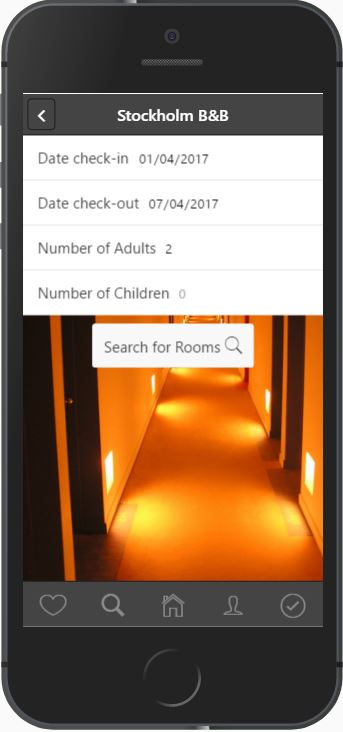
\includegraphics[width=.8\linewidth]{search.jpg}
  \caption{Söksteget}
  \label{fig:sfig2}
\end{subfigure}
\begin{subfigure}{.3\textwidth}
  \centering
  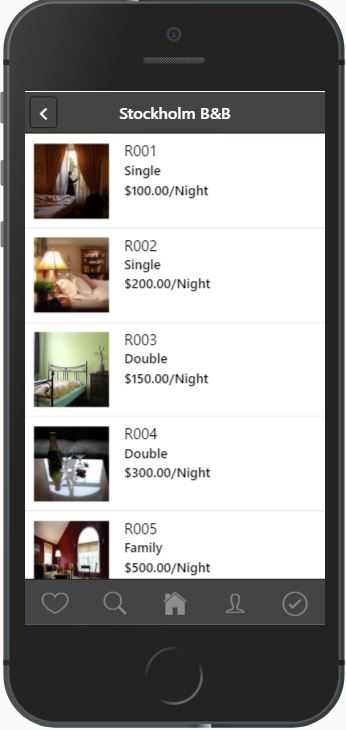
\includegraphics[width=.8\linewidth]{rooms.jpg}
  \caption{Rumsväljarsteget}
  \label{fig:sfig3}
\end{subfigure}\\


%second row
\begin{subfigure}{.3\textwidth}
  \centering
  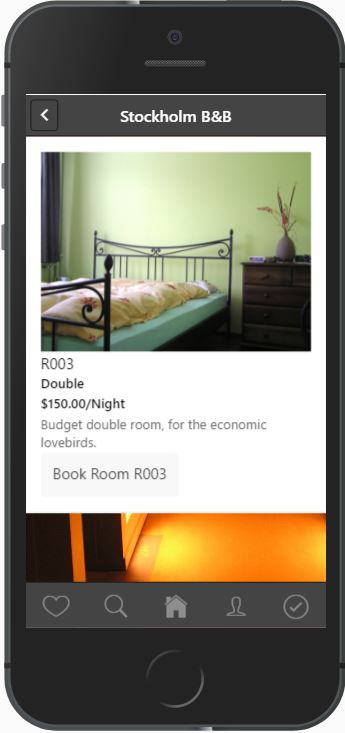
\includegraphics[width=.8\linewidth]{room.jpg}
  \caption{Rumsdetaljsteget}
  \label{fig:sfig4}
\end{subfigure}
\begin{subfigure}{.3\textwidth}
  \centering
  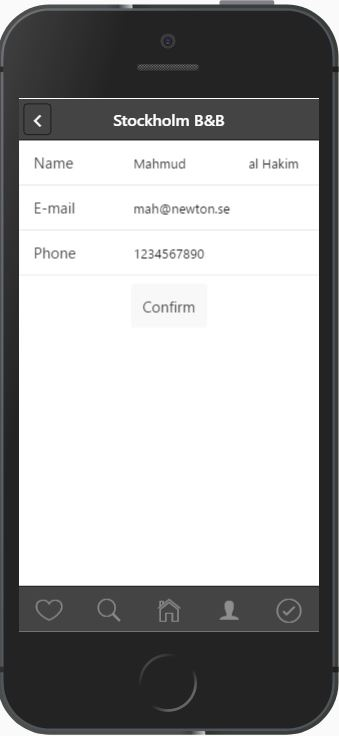
\includegraphics[width=.8\linewidth]{book.jpg}
  \caption{Bokningssteget}
  \label{fig:sfig5}
\end{subfigure}
\begin{subfigure}{.3\textwidth}
  \centering
  \includegraphics[width=.8\linewidth]{confirming.jpg}
  \caption{Konfirmationssteget}
  \label{fig:sfig6}
\end{subfigure}\\
\caption{De olika stegen i bokningsprocessen}
\label{fig:fig}
\end{figure}
\subsection{Inkapsling och åtkomst}
\label{encapsel}
Jag har valt att använda services för att spara undan data mellan vyerna. Jag har två services: En som sparar undan data när en användare söker efter lediga rum. En annan sparar sedan undan när man fyllt i sina uppgifter och vill bekräfta beställningen. Dessa består av getters och setters som sätter de variabler som behöver sparas mellan vyerna. Jag tyckte att detta var ett bra designval eftersom att det blir väldigt objektorienterat och inkapslat. \cite{exampleService}

\subsection{Felhantering och säkerhet}
Vid några tillfällen i flödet i applikationen har jag satt upp hinder för att användaren inte ska kunna utföra handlingar som skulle kunna orsaka problem. Till att börja med så är tab-navbaren inställd på disabled, dvs oklickbar. Detta är ett något kontroversiellt beslut, eftersom att många vill använda en nav-bar till att navigera, men detta är för att man inte ska kunna hoppa mellan stegen i flödet. På detta sätt så är det lättare att kunna kontrollera att alla information existerar i rätt ordning (tex antalet personer innan man bokar rum etc).

Vid tre tillfällen hindrar applikationen en ifrån att fortsätta om man inte har information ifrån föregående steg, två av dessa är ihopkopplade med de services som programmet använder sig av (se \ref{encapsel}).

Ytterligare en "failsafe" händer när man i bokningssteget går till konfirmationssteget.  Istället för att hämta informationen ifrån sökdatan i konfirmationsteget så hämtar man ifrån den datan som sparas i bokningssteget. Även om det i nuläget är omöjligt att gå till konfirmationssteget och sedan ändra sin sökning utan att gå genom bokningssteget så finns säkerheten där för att hantera en framtida ändring.\cite{failSafe}

Slutligen så i bokningssteget så får användaren respons på vad som saknas, på ett ungefär. Ifall epostadressen inte är korrekt ifylld, eller om något fält saknas så skrivs ett medelande ut på skärmen.

\section{Diskussion  och slutsats}
\subsection{Problem}
Under utvecklingens gång stötte jag på en del problem. Det mesta var rena kunskapsluckor i hur man man väljer ut en specifik lösning bland många generella för att lösa ett specifikt problem.

Till exempel så hittade jag flera olika sätt att skapa knappar, men dessa fungerade väldigt olika, och fungerade olika bra beroende på uppgiften de skulle utföra. Ionics documentation och eget experimenterande innehöll vital hjälp för att kunna urskilja mellan de olika varianternas fördelar och nackdelar.

Jag var ovan vid att använda services, och hade problem med att förstå vad de faktiskt gjorde och hur de skulle användas, men ganska snart så insåg jag hur likt det var objektoridenterad programmering, och jag kände mig då betydligt mer hemma i det tänket än i resten av angulars inline-scripting.

Filtrering är något som inte heller alltid sammarbetade med mig, men om man höll det ganska simpelt så var det betydligt lättare, så därför är inte filtren helt fantastika i koden.

Mycket av koden skulle kunna rensas upp och förbättras, och jag skulle vilja göra så att vissa tabbar låses upp av vissa aktioner av användaren.

\subsection{Lärdommar}
Jag ser tillbaka på projektet och inser att det inte var speciellt svårt. De mesta av problemen uppstod av min egna stress och av att jag inte lade ner tillräckligt med tid på projektet eller att förstå problemen som uppstod. Nyligen så har jag börjat ta steg för att förbättra min tidsoptimering, men de positiva effekterna av den kickade in lite sent för att jag skulle ha kunnat prestera fullt ut.

Jag använde git och github under \emph{hela} projektets gång, vilket visade sig vara väldigt värdefullt eftersom att det var betydligt lättare att testa sig fram.



\begin{thebibliography}{9}


\bibitem{exampleService}
Exempel på service:
\begin{lstlisting}
  .service('searchQuery', function () {
	/* this is not editable from the html nor the controller */
    var adultGuests = 1; 
/* but these are callable from the controller */
    this.getAdultGuests = function () {
      return adultGuests;
    };
    this.setAdultGuests = function (guests) {
      adultGuests = guests;
    };
  })
\end{lstlisting}

\bibitem{failSafe}
\begin{lstlisting}
    <ion-list>
      <!-- Prints a room which fits the room clicked on -->
      <ion-item ng-repeat='room in rooms
	| filter: {id : whichRoom}' class="item-text-wrap">
        <img ng-src="{{room.image}}" alt="{{room.name}}" width="100%" />
        <h2>{{room.id}}</h2>
{...}
        <!-- On book room, save the search. Why?
	Because if the user later will be able to
	go back multiple steps,
	it'll still be the last booked setup that is used -->
        <a href="#/tab/user" class="button"
	ng-click="setBookedRoom(room, getDates()[0], getDates()[1],
	getAdultGuests(), getChildGuests()); ">Book Room {{room.id}}</a>
      </ion-item>
    </ion-list>
\end{lstlisting}

\bibitem{github}
  https://github.com/Alicecold/BnB/tree/master/BnB

\end{thebibliography}

\end{document}